\chapter{Evaluation}

This chapter will evaluate the effectiveness of the compiler developed in this project, by comparing
the generated LLVM IR code and the performance of the compiled code against other compilers
utilising the LLVM as a backend. A quantitative analysis will be discussed first, followed by an
analysis on the limitations of the compiler as implemented, and potential improvements that could be
made.

\section{Software Testing}

To ensure the correctness of the compiler, as well as ensuring the requirements set out in
Chapter~\ref{ch:requirements} were met, a suite of unit tests were written to test the various
phases of the compiler. The unit tests were written using the ScalaTest framework, covering the
parser, enum refactor, IR generator, and closure conversion steps. The tests were written to cover a
range of scenarios, including edge cases. Where appropriate, mock objects were used to isolate the
unit under test from its dependencies (e.g. the generation of unique variable names).

Provided are example unit tests for the enum refactor stage:

\begin{code}{scala}
class EnumSpec extends AnyFlatSpec {
    // ... other tests ...

    behavior of "Match to If transformation"

    it should "correctly transform a match statement with a default case" in {
        val m = Match("a", List(MCase("A", "B", Num(6)), MCase("", "_", Num(5))))
        val expected = If(Op(Var("a"), "==", EnumRef("A", "B")), Num(6), Some(Num(5)))
        assert(transform_match_to_if(m) == expected)
    }

    it should "correctly transform a match statement with multiple cases" in {
        val m = Match("a", List(MCase("A", "B", Num(6)), MCase("C", "D", Num(5))))
        val expected = If(Op(Var("a"), "==", EnumRef("A", "B")), Num(6), Some(If(Op(Var("a"), "==", EnumRef("C", "D")), Num(5), Some(Op(Num(0), "+", Num(0))))))
        assert(transform_match_to_if(m) == expected)
    }

    it should "correctly transform a match statement with multiple cases and a default case" in {
        val m = Match("a", List(MCase("A", "B", Num(6)), MCase("C", "D", Num(5)), MCase("", "_", Num(4))))
        val expected = If(Op(Var("a"), "==", EnumRef("A", "B")), Num(6), Some(If(Op(Var("a"), "==", EnumRef("C", "D")), Num(5), Some(Num(4)))))
        assert(transform_match_to_if(m) == expected)
    }

    it should "correctly skip other cases after a default case" in {
        val m = Match("a", List(MCase("A", "B", Num(6)), MCase("", "_", Num(5)), MCase("C", "D", Num(4))))
        val expected = If(Op(Var("a"), "==", EnumRef("A", "B")), Num(6), Some(Num(5)))
        assert(transform_match_to_if(m) == expected)
    }
}
\end{code}

As seen, the tests are written in a BDD (Behaviour-driven development) style, with each test case
describing the expected behaviour of the function under test. In total, 50 unit tests were written
to test the various phases of the compiler.

End-to-end testing was used to evaluate the LLVM IR output. A suite of test programs
were written to test the various features of the language, including functions, structs, enums, and
closures. The test programs were compiled using the project compiler, and the output LLVM IR code
was manually inspected and executed to ensure that the programs produced the correct output.

% TODO tests

\section{Performance Benchmarking}

A key language feature ubiquitous in functional programming languages is the ability to define
recursive functions. A pure functional language paradigm will utilise recursion as a primary method
of iteration, as opposed to the traditional imperative loop constructs. Therefore, the ability for a
compiler to optimise recursive functions is crucial for the performance of the generated code.

The Ackermann function is a recursive computable function that grows rapidly with respect to its
inputs, and is a classic example used to benchmark the ability of a compiler to optimise recursive
calls.

The Ackermann function is defined as follows:

\singlespacing
\vspace{-0.7cm}
\begin{align*}
    ack(m, n) = \begin{cases}
        n + 1 & \text{if } m = 0 \\
        ack(m - 1, 1) & \text{if } m > 0 \text{ and } n = 0 \\
        ack(m - 1, ack(m, n - 1)) & \text{if } m > 0 \text{ and } n > 0
    \end{cases}
\end{align*}
\doublespacing

Despite the only arithmetic operation being an addition or subtraction of one, even small inputs
such as $ack(4,2)$ result in a value of $2 \times 10^{19728}$ due to the nested recursion, implying
that the output value of the function is indicative of the running time of the function itself.
Without proper optimisation, the Ackermann function can quickly exhaust the call stack, and result
in a stack overflow error. For evaluation purposes, the Ackermann function will be tested with $m=3$
to restrict function growth to (at most) exponential.

To properly evaluate the performance of the project compiler, the generated LLVM IR code was
compiled to a binary using the LLVM compiler (\texttt{llc}), and then linked against the C standard
library \texttt{libc} using the GNU Compiler Collection (\texttt{gcc}). Linking against
\texttt{libc} is necessary to provide the required \texttt{printf} function for output, as it not
defined in the LLVM. The resulting binary was then executed to measure the time taken to compute the
Ackermann function for various values of $n$.

The project compiler was benchmarked against Haskell (compiled with GHC), and C (compiled with
Clang). Haskell was chosen as a comparison due to its functional programming nature that has a
compiler compatible with the LLVM backend. C was chosen due to its high performance, and high
compatibility with the LLVM. (The LLVM was originally developed for C and C++ in
mind.~\autocite{lattner2004llvm})

Below is the implementation of the Ackermann function in all three languages:

\vspace{0.3cm}
\begin{tcbitemize}[raster columns=3, raster equal height=rows,size=small,space to upper]
    \tcbitem
        \footnotesize
        \begin{minted}{scala}
            def ack(m:Int, n:Int): Int =
                if m == 0 then
                    n+1
                else if n == 0 then
                    ack(m-1, 1)
                else
                    ack(m-1, ack(m, n-1));

            def main() = {
                print(ack(3,10))
                0
            }
        \end{minted}
        \tcblower
        \footnotesize $ack(m, n)$ in the project.
    \tcbitem
        \footnotesize
        \begin{minted}{haskell}
            ack :: Int -> Int -> Int
            ack 0 n = n+1
            ack m 0 = ack (m-1) 1
            ack m n = ack (m-1) (ack m (n-1))

            main = print (ack 3 10)
        \end{minted}
        \vfill
        \tcblower
        \footnotesize $ack(m, n)$ in Haskell.
    \tcbitem
        \scriptsize
        \begin{minted}{c}
            #include <stdio.h>

            int ack(int m, int n) {
                if (m == 0) {
                    return n+1;
                } else if (n == 0) {
                    return ack(m-1, 1);
                } else {
                    return ack(m-1, ack(m, n-1));
                }
            }

            int main() {
                printf("%d\n", ack(3, 10));
                return 0;
            }
        \end{minted}
        \tcblower
        \footnotesize $ack(m, n)$ in C.
\end{tcbitemize}
\vspace{0.4cm}

To ensure a fair comparison, and to evaluate the effect of the LLVM toolchain on compiler frontends,
all compilers were compiled at two optimisation levels: \texttt{-O0} and \texttt{-O3}. The
\texttt{-O0} flag disables all optimisations, while the \texttt{-O3} flag enables all
optimisations\footnote{The GHC compiler actually needs two flags to enable all optimisations; one
for GHC (\texttt{-O2}), and one for the LLVM (\texttt{-optlc-O3}).}.

Each compiler was benchmarked ten times with $ack(3,n)$ for each input value of $n$ (ranging from 10
to 15 inclusive) across both optimisation levels, and the average time taken was recorded. Results
were obtained on a machine with an Intel Core i7-13620H CPU and 32GB of RAM, running Ubuntu 22.04.4
under WSL2. The results of the benchmark are shown in Table~\ref{tab:ackermann-benchmark}, and
graphed in Figure~\ref{fig:ackermann-benchmark}.


\subsection{Results}

\begin{table*}\centering
    \renewcommand{\arraystretch}{1.3}
    \label{tab:ackermann-benchmark}
    \caption{Ackermann function benchmark results (in seconds)}

    \begin{tabular}{@{}lcccccccc@{}} \toprule
        Lang        & \multicolumn{2}{c}{Project} &              & \multicolumn{2}{c}{C} &              & \multicolumn{2}{c}{Haskell}                                  \\
        \cmidrule{2-3} \cmidrule{5-6} \cmidrule{8-9}
                    & \texttt{-O0}                & \texttt{-O3} &                       & \texttt{-O0} & \texttt{-O3}                &  & \texttt{-O0} & \texttt{-O3} \\ \midrule
        $ack(3,10)$ & 0.080                       & 0.024        &                       & 0.120        & 0.024                       &  & 1.334        & 0.101        \\
        $ack(3,11)$ & 0.312                       & 0.093        &                       & 0.490        & 0.092                       &  & 5.449        & 0.387        \\
        $ack(3,12)$ & 1.267                       & 0.370        &                       & 1.976        & 0.366                       &  & 22.63        & 1.578        \\
        $ack(3,13)$ & 5.071                       & 1.502        &                       & 8.088        & 1.495                       &  & 99.05        & 6.540        \\
        $ack(3,14)$ & 20.75                       & 6.193        &                       & 32.90        & 6.130                       &  & 475.3        & 28.08        \\
        $ack(3,15)$ & --                          & 24.74        &                       & --           & 23.26                       &  & 2237         & 127.1        \\
        \bottomrule
    \end{tabular}
\end{table*}

\begin{figure}[t]
    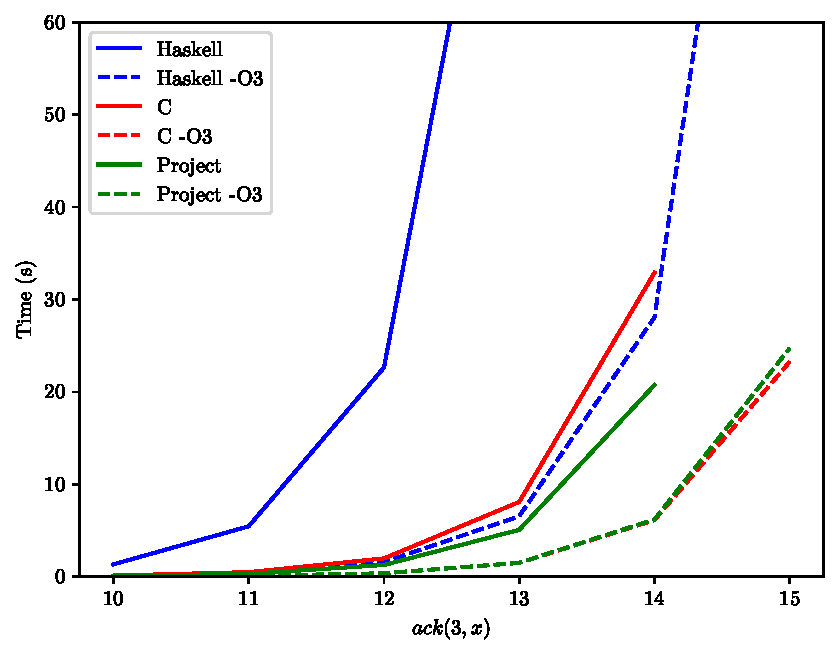
\includegraphics{Graphics/ackermann-benchmark.pdf}
    \caption{A graph reflecting the results of the Ackermann function benchmark.}
    \label{fig:ackermann-benchmark}
\end{figure}

The results show that, at optimisation level \texttt{-O0}, the
project compiler performs significantly better than Haskell, and slightly better than C across all
test cases.

On analysing the generated LLVM IR code, Clang (at \texttt{-O0}) appears to copy all function
arguments to the stack as local variables before using them, occurring for each function invocation.
This results in many \texttt{alloca}, \texttt{store} and \texttt{load} instructions being called per
function call. The project compiler, on the other hand, utilises the LLVM's SSA form to eliminate
unnecessary memory operations, and instead uses the function arguments directly. This results in
significantly fewer memory related instructions, and a more efficient program as reflected by the
results.

A common behaviour observed in both the project compiler and Clang is the failure to compute the
Ackermann function for $ack(3,15)$, terminating with a segmentation fault. This is due to the
Ackermann function rapidly exhausting the call stack from the nested recursion. The project compiler
does not have an implementation for tail call optimisation, and Clang does not enable it by default.

On the other hand, the Haskell compiler is able to compute the function for $ack(3,15)$ without any
optimisations. This is likely due to Haskell's lazy evaluation strategy, as it does not create stack
frames on each function call, but when an unevaluated value (a `thunk') is evaluated. Due to this
lack of a traditional call stack, Haskell is able to compute the Ackermann function without running
out of stack space.

At optimisation level \texttt{-O3}, all compilers expectedly perform better than at \texttt{-O0},
but at different rates. The project compiler sees approximately a 3.3x improvement in performance, C
sees a 5x improvement, and Haskell sees a 14x improvement. The project compiler now performs almost
identically with C for small inputs, slightly dropping off as $n$ increases. Haskell, however, still
performs significantly worse than the other two compilers, as the GHC compiler appears to struggle
optmising for this particular function.

The generated LLVM IR code for the project compiler and Clang are now very similar, with both
utilising tail call optimisation to reduce the number of recursive calls inside the Ackermann
function down to one. This results in a significant reduction in the number of stack frames
required, and allows the function to be computed for larger inputs, such as $ack(3,15)$. This also
explains the very similar performance of the two compilers at \texttt{-O3}, as both compilers are
able to leverage the LLVM's optimisation passes to generate efficient code.

Despite primitive nature of the project compiler compared to other well-established compilers, the
results of the benchmark show that by leaning on the LLVM toolchain to perform optimisations, the
project compiler is able to generate efficient code in-line with other compilers utilising the LLVM
as a backend. Certain optmisiations such as tail call optimisation can be leveraged `for free'
without the need to implement them in the compiler itself.

\section{Limitations}

It is near impossible to claim any compiler is perfectly implemented against the specification and
semantics of a language. This project is no exception, and due to time constraints has a number of
limitations that prevent it from being considered a complete compiler. There are also additional
functional programming features that could be implemented to improve the experience of the end-user.
The following sections will discuss some specific limitations of the project compiler, and potential
improvements that could be made.

\subsection{Sum Types}

While the compiler supports enumerated types, the more general concept of sum types (also known as
tagged unions) are not supported. Sum types are a common feature of functional programming languages
-- particularly when paired with pattern matching -- and are used to represent a value that can take
on one of several different forms.

For example, a sum type in Rust can be defined as follows:

\begin{code}{rust}
    enum Foo {
        Bar(bool),
        Baz(i32)
    }
\end{code}

Note that the type \texttt{Foo} can take on one of two forms: \texttt{Bar} with a boolean value, or
\texttt{Baz} with an integer value. This differs from the enumerated types supported by the project
compiler, which can only take on one of a fixed set of integer values.

Support for sum types cannot be implemented using the same method as enums, as the value of a sum
type is not known at compile time. Rather, multiple LLVM structures would need to be generated:

\begin{code}{llvm}
    %Foo = type { i8, [4 x i8] } ; tag, data
    %Foo_Bar = type { i8, i1 }   ; tag (0), boolean
    %Foo_Baz = type { i8, i32 }  ; tag (1), integer
\end{code}

The base type, \texttt{Foo}, would contain an integer `tag' to indicate which variant of the sum
type it is, and an array of bytes to store the data associated with the variant. The
\texttt{Foo_Bar} and \texttt{Foo_Baz} types represent the exact layout of the data for each variant.
Creating a variant of type \texttt{Foo} would require allocating memory for the base type, setting
the tag to the appropriate value for the variant, bitcasting the memory address to the appropriate
variant type, and then storing the data in the appropriate field. Likewise, extracting the data from
a value of type \texttt{Foo} would require branching on the tag, bitcasting the value to the
appropriate variant type depending on the tag, and then extracting the data from the appropriate
fields.

As can be seen, implementing sum types is not trivial, and would not only require a refactor of the
code generation phase, but also a redesign of the type system to support the additional complexity
of sum types.

\subsection{Type System}

The project compiler has a very basic type system, and does not support many of the features found
in more advanced type systems. For example, the type system does not support type inference or
polymorphic types. The type system also does not support type classes, which are used to define a
set of functions that can be implemented for a type, and are used to provide ad-hoc polymorphism.
A more robust type system would allow for more primitives to be defined, and would allow for more
expressive programs to be written.

Implementing a more advanced type system would require a significant refactor of the type checker
phase, and would require a redesign of the type checker to support the additional complexity of the
type system. It would also require the implementation of additional type checking rules to support
the new features of the type system. As mentioned earlier, the Hindley-Milner type inference
algorithm could be implemented to provide type inference for the project compiler. This would allow
the compiler to infer the types of variables and expressions without requiring the user to provide
explicit type annotations.

\subsection{Heap-allocated variables}

The project compiler does not support heap-allocated variables. All variables are stack-allocated,
and are deallocated when they go out of scope. This can be problematic for programs that require
variables to persist beyond the scope in which they were defined, such as returning a struct from a
function. Additionally, the implementation of data structures based on lists (e.g. Strings) is
limited without heap-allocated variables, as the size of the list must be known at compile time.

\begin{tcolorbox}
    \begin{minted}{scala}
        def make_pair(a: Int, b: Int): Pair = Pair(a, b)

        def main() = {
            val p = make_pair(1, 2)
            print(p.b)
            0
        }
    \end{minted}
    \tcblower
    \footnotesize
    The output for this program might not be \texttt{2} as expected. This is undefined behaviour, as
    the pair returned in \texttt{make\_pair} is deallocated when it returns and falls out of scope.
\end{tcolorbox}

Adding support for heap-allocated variables would require a refactor of the code generation phase.
The phase would need to be modified to allocate and deallocate memory on the heap, ensuring that
memory is not leaked or accessed after it has been deallocated (dangling pointers). Without
providing explicit functions for memory management like \texttt{malloc} and \texttt{free} to the
end-user, this would need be implemented in the form of a garbage collector.

